\begin{figure}[htb!]
    \centering
    \begin{tabular}{c}
        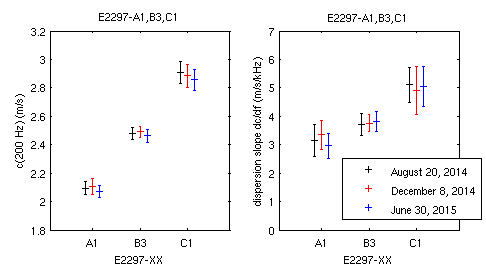
\includegraphics[width=0.75\linewidth]{figs/phase2_longitudinal_stability.png} \\
        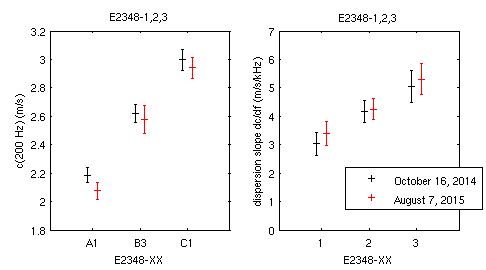
\includegraphics[width=0.75\linewidth]{figs/phaseIIset2_temporal_stability.png} \\
    \end{tabular}
    \caption{Results for the quantities $c_{200}$ (left) and dispersion slope
        $\frac{dc}{df}$ (right) for phantoms [TOP ROW] E2297-A1, B3, and C1
        from measurements made on August 20, 2014 (black), December 8, 2014
        (red), and June 30, 2015 (blue) and [BOTTOM ROW] E2348-1, -2, and -3
        from October 16, 2015 and August 07, 2015. The data points represent
        the mean $\pm$ standard deviation from 16 measurements in each
        phantom.} \label{fig:phase2_longitudinal_stability}
\end{figure}
